\documentclass[tikz,border=10pt]{standalone}
\usetikzlibrary{matrix, positioning, fit, backgrounds, decorations.pathreplacing}

\begin{document}
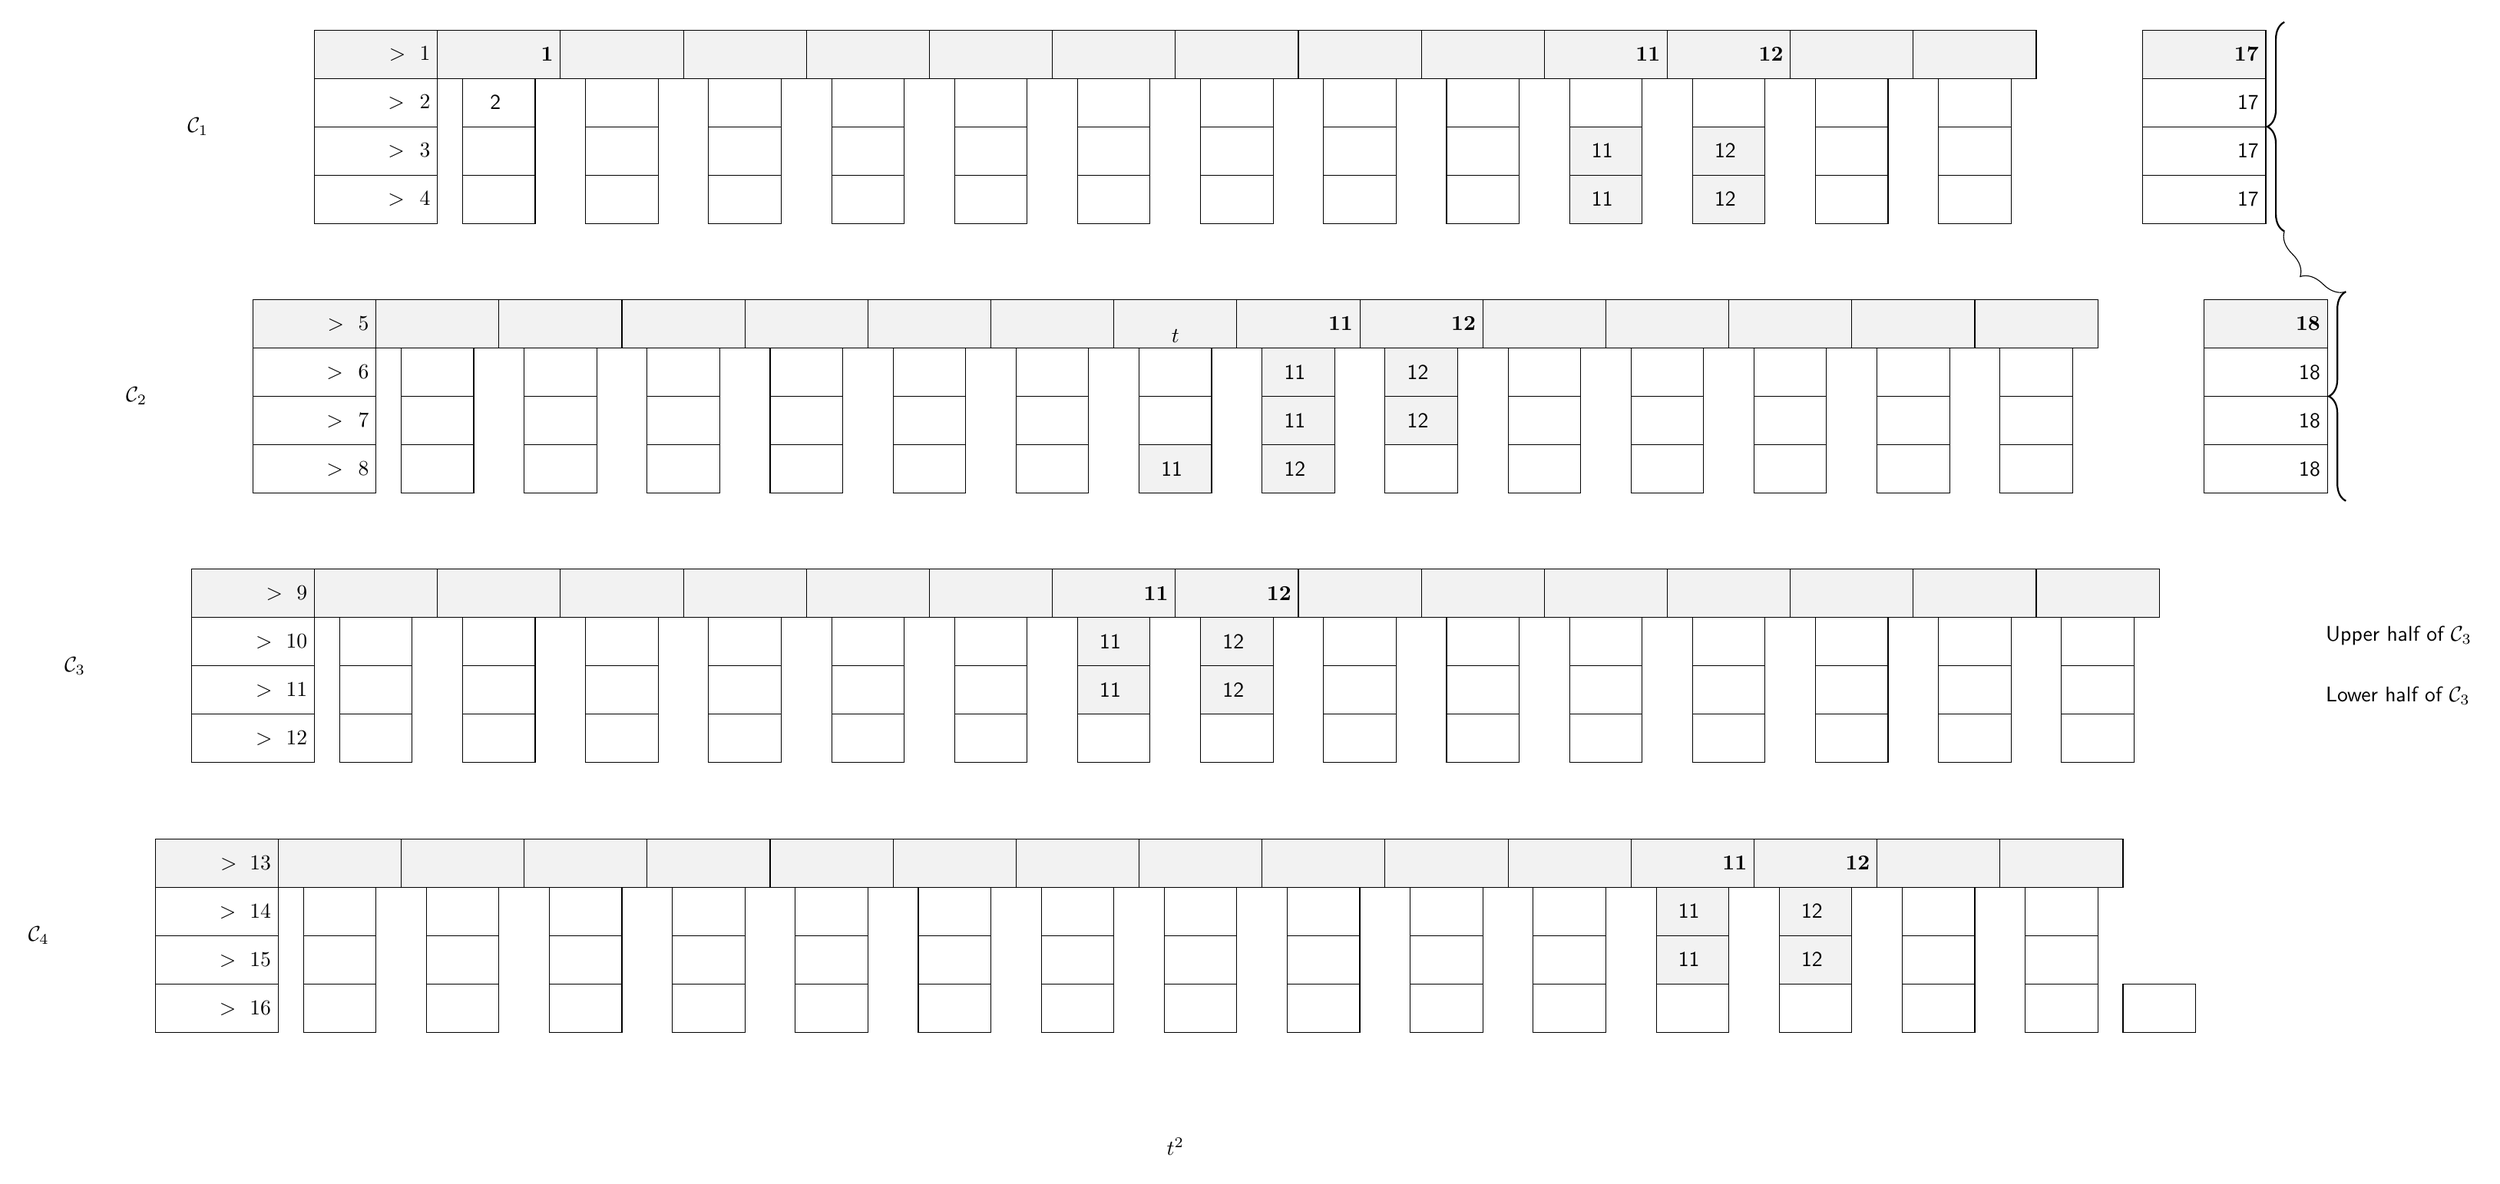
\begin{tikzpicture}[scale=1, font=\sffamily]

% Define styles for the matrix nodes
\tikzset{
    table/.style={
        matrix of nodes,
        nodes in empty cells,
        row sep=-\pgflinewidth,
        column sep=-\pgflinewidth,
        nodes={
            minimum width=1.2cm,
            minimum height=0.8cm,
            anchor=center,
            draw,
            align=center
        },
        column 1/.style={nodes={text width=1.8cm, align=right}},
        row 1 column 1/.style={nodes={minimum width=1.8cm}},
    },
    header/.style={
        text width=1.8cm,
        align=right,
        draw,
        minimum height=0.8cm,
        fill=gray!10,
        anchor=center,
        font=\bfseries
    },
    largebrace/.style={
        decorate,
        decoration={brace, amplitude=8pt},
        thick
    }
}

% Draw the first table
\matrix[table, name=M1, row 1/.style={nodes={header}}] at (0,0) {
    $>1$ & |[fill=gray!10]| 1 &&&&&&&&& |[fill=gray!10]| 11 & |[fill=gray!10]| 12 & & \\
    $>2$ & 2 &&&&&&&&&&&& \\
    $>3$ & &&&&&&&&& |[fill=gray!10]| 11 & |[fill=gray!10]| 12 & & \\
    $>4$ & &&&&&&&&& |[fill=gray!10]| 11 & |[fill=gray!10]| 12 & & \\
};

% Label the left side
\node[align=left, anchor=east, left=1cm of M1, xshift=-0.5cm] (C1) {$\mathcal{C}_1$};

% Draw the second table
\matrix[table, name=M2, row 1/.style={nodes={header}}, below=of M1] {
    $>5$ & &&&&&&& |[fill=gray!10]| 11 & |[fill=gray!10]| 12 & &&&& \\
    $>6$ & &&&&&&& |[fill=gray!10]| 11 & |[fill=gray!10]| 12 & &&&& \\
    $>7$ & &&&&&&& |[fill=gray!10]| 11 & |[fill=gray!10]| 12 & &&&& \\
    $>8$ & &&&&&& |[fill=gray!10]| 11 & |[fill=gray!10]| 12 & &&&&& \\
};

% Label the left side
\node[align=left, anchor=east, left=1cm of M2, xshift=-0.5cm] (C2) {$\mathcal{C}_2$};

% Draw the third table
\matrix[table, name=M3, row 1/.style={nodes={header}}, below=of M2] {
    $>9$ & &&&&&& |[fill=gray!10]| 11 & |[fill=gray!10]| 12 & &&&&&& \\
    $>10$ & &&&&&& |[fill=gray!10]| 11 & |[fill=gray!10]| 12 & &&&&&& \\
    $>11$ & &&&&&& |[fill=gray!10]| 11 & |[fill=gray!10]| 12 & &&&&&& \\
    $>12$ & &&&&&&&&&&&&&& \\
};

% Label the left side
\node[align=left, anchor=east, left=1cm of M3, xshift=-0.5cm] (C3) {$\mathcal{C}_3$};

% Draw the fourth table
\matrix[table, name=M4, row 1/.style={nodes={header}}, below=of M3] {
    $>13$ & &&&&&&&&&&& |[fill=gray!10]| 11 & |[fill=gray!10]| 12 & & \\
    $>14$ & &&&&&&&&&&& |[fill=gray!10]| 11 & |[fill=gray!10]| 12 & & \\
    $>15$ & &&&&&&&&&&& |[fill=gray!10]| 11 & |[fill=gray!10]| 12 & & \\
    $>16$ & &&&&&&&&&&&&&& & \\
};

% Label the left side
\node[align=left, anchor=east, left=1cm of M4, xshift=-0.5cm] (C4) {$\mathcal{C}_4$};

% Add t1 label at bottom of the tables
\node[below=of M1, yshift=-0.5cm] {$t$};

% Add t2 label at bottom of the tables
\node[below=of M4, yshift=-0.5cm] {$t^2$};

% Draw the vertical bars on the right
\foreach \i/\j in {1/17, 2/18}
{
    \matrix[table, name=V\i, right=1.5cm of M\i, row 1/.style={nodes={header}}] {
        \j \\
        \j \\
        \j \\
        \j \\
    };
}

% Label the upper half of C3
\node[right=1.5cm of M3, xshift=1cm, yshift=0.5cm, align=left] (upper_label) {Upper half of $\mathcal{C}_3$};

% Label the lower half of C3
\node[right=1.5cm of M3, xshift=1cm, yshift=-0.5cm, align=left] (lower_label) {Lower half of $\mathcal{C}_3$};

% Draw the braces
\draw[largebrace, decorate, thick] ([xshift=5pt]V1.south east) -- node[right=10pt] {} ([xshift=5pt]V1.north east);
\draw[largebrace, decorate, thick] ([xshift=5pt]V2.south east) -- node[right=10pt] {} ([xshift=5pt]V2.north east);
\draw[decorate, decoration={brace, mirror, amplitude=10pt}] ([xshift=5pt]V1.south east) -- node[right=15pt, align=left] {} ([xshift=5pt]V2.north east);

\end{tikzpicture}
\end{document}